\documentclass{article}[11pt]
\usepackage{blindtext}
\usepackage{graphicx}
\usepackage{enumitem}
\usepackage{amssymb}
\usepackage{amsthm}
\usepackage{amsmath}
\usepackage{graphicx}
\usepackage{MnSymbol}
\usepackage{wasysym}
\usepackage{pgfplots}
\usepackage{tikz}
\usetikzlibrary{calc}
\usetikzlibrary{shapes}
\usetikzlibrary{shapes.geometric}
\usepgfplotslibrary{fillbetween}
\pgfplotsset{width=10cm,compat=1.9}

\title{The Painter's Paradox and Gabriel's Horn}
\author{Barnett Yang}
\date{April 2, 2021}

\begin{document}

\maketitle
\section*{Introduction: Mathematics and Paradoxes}
One of the most fascinating aspects of mathematics is mathematical paradoxes. While some paradoxes seem to truly defy conventional logic (see the Banach-Tarski paradox for more), other so-called paradoxes can be classified more accurately as "unexpected results"--results that may be unintuitive yet make mathematical sense to most people. While the Painter's Paradox is one of these "half-paradoxes," it nevertheless serves as a nice foray into the volumes and surface areas of solids of revolution.

\section{Gabriel's Horn}
Consider the graph of $f(x) = \frac{1}{x}$ below and the region bounded by the x-axis, $f(x)$, and $x=1$. Note how this region extends into infinity.

\begin{center}
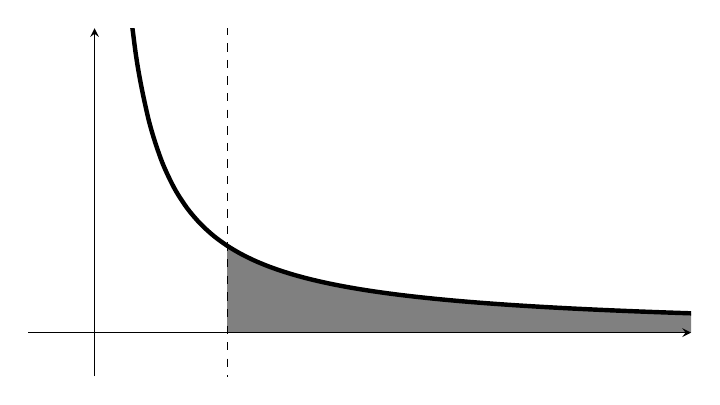
\begin{tikzpicture}
    \begin{axis}[
        xmin=-0.5, xmax=4.5,
        ymin=-0.5, ymax=3.5,
        axis lines=center,
        axis on top=true,
        domain=0.1:10,
        samples=100,
        height=6cm,
        width=10cm,
        ticks=none,
        style={font=\LARGE}
    ]
        \fill [gray, domain=1:6, variable=\x]
        (1, 0)
        -- plot ({\x}, {1/\x})
        -- (6, 0)
        -- cycle;
        \addplot[smooth, ultra thick, name path=A]{1/x} node[above]{$\frac{1}{x}$};
        \addplot[draw=none, name path=B]{0};
        \addplot[gray] fill between[of=A and B,soft clip={domain=1:6}];
        \addplot [dashed] coordinates {(1, 6) (1, -1)} node[right]{$x=1$};
    \end{axis}
\end{tikzpicture}
\end{center}

It is a relatively elementary mathematical exercise to show that this area is infinite:
\begin{align*}
\lim_{t \to \infty}\int_1^{t}\frac{1}{x}\textrm{d}{x} &= \lim_{t\to\infty}[\ln{x}]_{x=1}^{x=t} \\
&= \lim_{t\to\infty}{\ln{t}} - 0 \\
&= \infty
\end{align*}

I am intentionally begin verbose with my limit notation. In calculus, there is no concept of infinity as a limit of integration. The proper way to take an infinite integral is to assign a variable as an upper limit of integration and have that variable approach infinity.

More interesting is to consider the properties of the solid generated by revolving the aforementioned bounded region about the x-axis. Doing so results in the figure graphed below:
\hspace{11pt}

\begin{center}
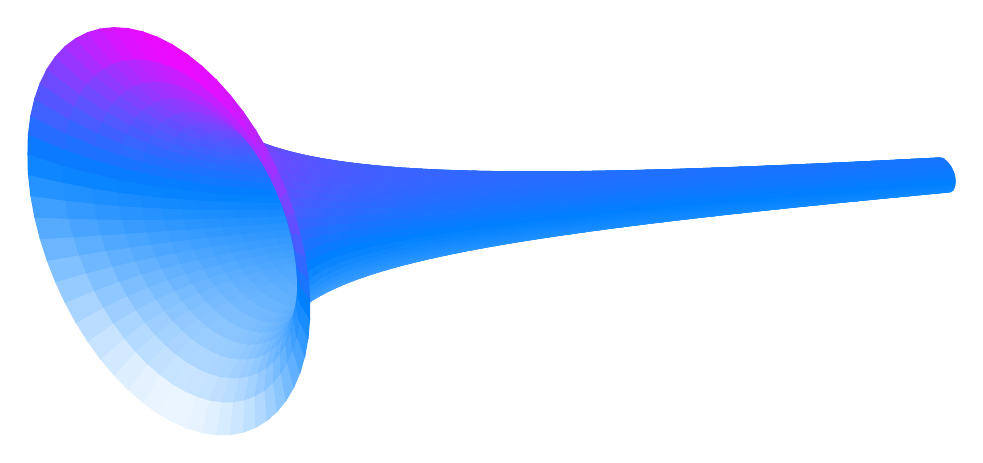
\begin{tikzpicture}
    \begin{axis}[
        axis lines=none,
        colormap/cool,
        view={-20}{20},
        height=10cm,
        width=15cm
    ]
    \addplot3[surf,shader=flat,
        samples=60,
        domain=1:12,y domain=0:2*pi,
        z buffer=sort
    ]
    (x,{(1/x) * cos(deg(y))}, {(1/x) * sin(deg(y))});
    \end{axis}
\end{tikzpicture}
\end{center}

Due to its horn-like shape, mathematicians have bestowed upon this solid the name "Gabriel's Horn." (Unfortunately, this does not mean you'll meet Angel Gabriel any time soon; he's at the impossibly narrow end of this impossibly long horn that is life.) From Gabriel's Horn arises the famous Painter's Paradox. While the solid of revolution generated by $f(x) = \frac1x$ has finite volume, its surface area is infinite. In other words, if a painter were to treat the horn as a paint bucket, they could quite easily fill it up with paint. However, no matter how hard they tried, no painter would ever be able to paint the exterior of Gabriel's Horn in a finite amount of time.

As always, with any mathematical assertion comes a proof. So let's go ahead and use the next two sections to prove the Painter's Paradox!

\section{Painter's Paradox Part I: The Volume of Gabriel's Horn}
To find the volume of Gabriel's Horn, we can imagine summing together an infinite number of disks each with an infinitely small thickness that we will call $\textrm{d}x$, which is also the change in our x-value between disks. Note that each disk in our summation is a cylinder with height $\textrm{d}x$ and radius $f(x)$.

\begin{center}
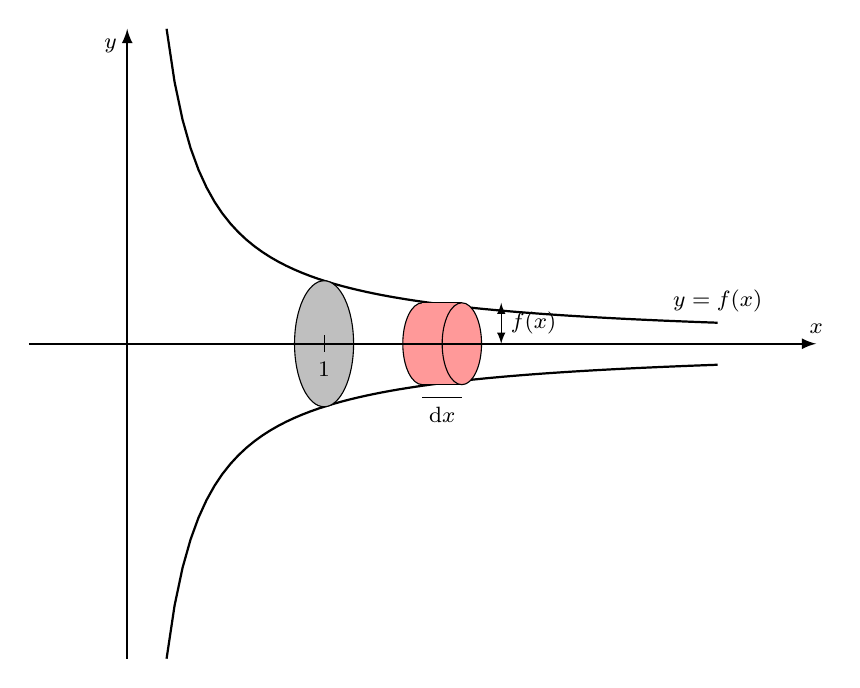
\begin{tikzpicture}[scale=1,>=latex,x=2.5cm,y=0.8cm]
    \draw[-,thick,domain=0.2:3,samples=70] plot (\x,{1/\x}) node[above] {\footnotesize $y=f(x)$};
    \draw[-,thick,domain=0.2:3,samples=70] plot (\x,{-1/\x});
    \draw[fill=gray!50] (1,0) circle [x radius =.15 , y radius =1];
    \draw[fill=red!40] (1.5,0) circle [x radius =.1 , y radius = 0.65];
    \fill[red!40] (1.5,-0.65) rectangle (1.7,0.65);
    \draw[fill=red!40] (1.7,0) circle [x radius =.1 , y radius = 0.65];
    \draw (1.5,0.65) -- (1.7,0.65);
    \draw (1.5,-0.65) -- (1.7,-0.65);
    \draw[] (1.5,-0.85) -- (1.7,-0.85) node[below, midway] {\footnotesize $\textrm{d}x$};
    \draw[<->] (1.9,0) -- (1.9,0.65) node[right, midway]  {\footnotesize $f(x)$};
    \draw[->,thick] (-0.5,0) -- (3.5,0) node[above] {\footnotesize $x$};
    \draw[->,thick] (0,-5) -- (0,5) node[below left]{\footnotesize $y$};
    \draw[-] (1,3pt) -- (1,-3pt) node[below] {\footnotesize $1$};
\end{tikzpicture}
\end{center}

To find the total volume, we can simply find an expression for a single slice of our volume and them sum the slices together across the interval $[1, \infty)$. Based on the diagram of a single disk below, we can easily see that the volume of each infinitely thin cylinder is $\frac{\pi\textrm{d}x}{x^2}$.

\begin{center}
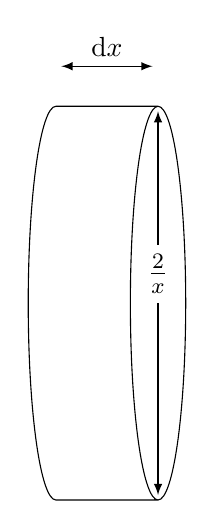
\begin{tikzpicture}[>=latex,shorten >=2pt,shorten <=2pt,shape aspect=3]
    \node (A) [cylinder, draw, minimum height=2cm, minimum width=5cm] {};
    \draw [<->] (A.before top) -- (A.after top) node [midway, above,fill=white] {\large $\frac2x$};
    \coordinate(htop) at ($(A.before top)!-1*.1!(A.after top)$);
    \coordinate(hbot) at ($(A.after bottom)!-1*.1!(A.before bottom)$);
    \coordinate(hlab) at ($(htop)!.5!(hbot)+(A.north)!.9!(A.center)$);
    \draw[<->] (hbot)--(htop);
    \path (hlab) node {$\textrm{d}x$}; %Modify height label here
\end{tikzpicture}
\end{center}

Integrating, we find the total volume:

\begin{align*}
    \lim_{t \to \infty}\int_1^{t}\frac{\pi}{x^2}\textrm{d}x &= \pi\lim_{t \to \infty}\int_1^{t}\frac{1}{x^2}\textrm{d}x \\
    &= -\pi \lim_{t \to \infty}[\frac1x]_{x=1}^{x=t} \\
    &= -\pi (\lim_{t \to \infty}\frac1t - 1) \\
    &= \pi
\end{align*}

Very nice! So we have a finite volume of $\pi$ for our solid of revolution.

\section{Painter's Paradox Part II: The Surface Area of Gabriel's Horn}
Now let's consider a slightly harder problem: finding the surface area of Gabriel's Horn. For this problem, we can consider taking our solid of revolution and splitting it into infinitely many conical \emph{frustums}, each with infinitely small thickness $\textrm{d}x$. From there, we can sum the lateral surface area of each frustum to get the total surface area of Gabriel's Horn.

\begin{center}
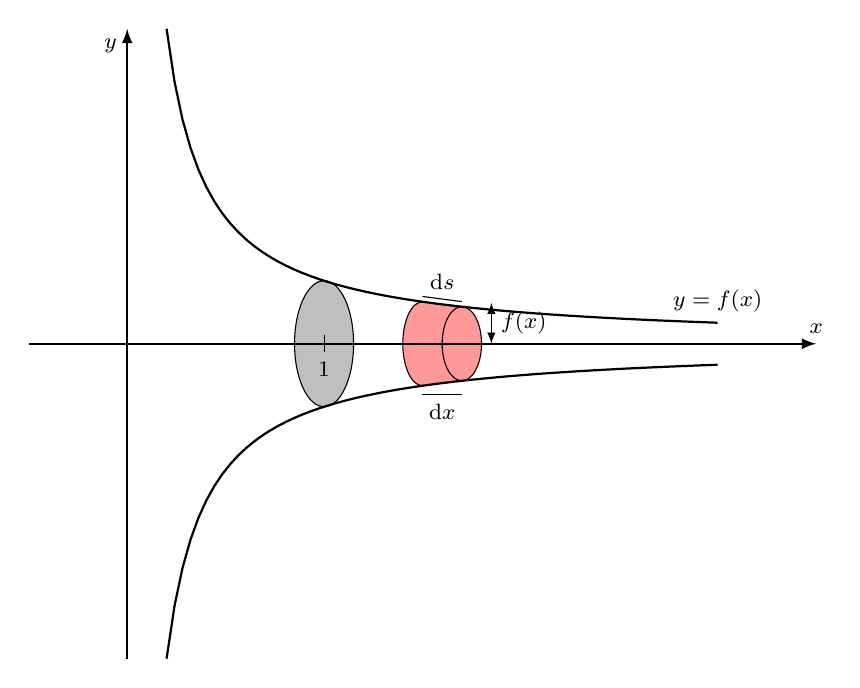
\begin{tikzpicture}[scale=1,>=latex,x=2.5cm,y=0.8cm]
    \draw[fill=gray!50] (1,0) circle [x radius =.15 , y radius =1];
    \draw[fill=red!40] (1.5,0) circle [x radius =.1 , y radius = 0.66666666];
    \node[
        trapezium, 
        draw=none, 
        fill=red!40, 
        anchor=south,
        rotate=-90, 
        trapezium left angle=86, 
        trapezium right angle=86,
        minimum width=1.08cm,
        trapezium stretches=true,
        minimum height=.5cm
    ](t) at (1.5, 0) {};
    \draw[fill=red!40] (1.70,0) circle [x radius =.1 , y radius = 0.58823529];
    \draw[-,thick,domain=0.2:3,samples=70] plot (\x,{1/\x}) node[above] {\footnotesize $y=f(x)$};
    \draw[-,thick,domain=0.2:3,samples=70] plot (\x,{-1/\x});
    \draw[] (1.5,-0.80) -- (1.70,-0.80) node[below, midway] {\footnotesize $\textrm{d}x$};
    \draw[] (1.5,0.75) -- (1.70,0.67) node[above, midway] {\footnotesize $\textrm{d}s$};
    \draw[<->] (1.85,0) -- (1.85,0.65) node[right, midway]  {\footnotesize $f(x)$};
    \draw[->,thick] (-0.5,0) -- (3.5,0) node[above] {\footnotesize $x$};
    \draw[->,thick] (0,-5) -- (0,5) node[below left]{\footnotesize $y$};
    \draw[-] (1,3pt) -- (1,-3pt) node[below] {\footnotesize $1$};
\end{tikzpicture}
\end{center}

Note that each frustum located at $x=x_0$ has two radii: one is determined by the value of the function $f(x) = \frac1x$ at $x=x_0$ (i.e. has radius $\frac1{x_0}$) and the other is determined by the value of the function at $x=x_0+\textrm{d}x$ (i.e. has radius $\frac1{x_0+\textrm{d}x}$). The frustum also has lateral height $\textrm{d}s$, which is the infinitesimal \emph{arc length} from $x_0$ to $x_0 + \textrm{d}x$. In other words, $\textrm{d}s$ is the distance between the two points $(x_0, f(x_0))$ and $(x_0 + \textrm{d}x, \frac1{x_0 + \textrm{d}x})$.

\begin{center}
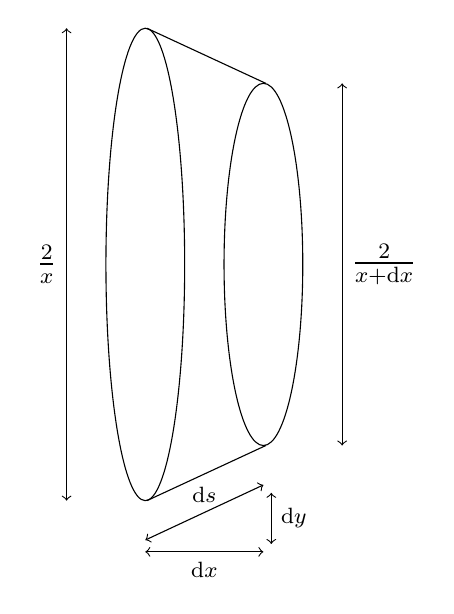
\begin{tikzpicture}[scale=1]
    \draw[] (0,0) circle [x radius =.5 , y radius = 3];
    \draw[] (0.02, 3) -- (1.53, 2.3);
    \draw[] (0.02, -3) -- (1.53, -2.3);
    \draw[] (1.50,0) circle [x radius =.5 , y radius = 2.3];
    \draw[<->] (0, -3.5) -- (1.5, -2.8) node[above, midway] {\footnotesize $\textrm{d}{s}$};
    \draw[<->] (0, -3.65) -- (1.5, -3.65) node[below, midway] {\footnotesize $\textrm{d}{x}$};
    \draw[<->] (1.6, -2.9) -- (1.6, -3.55) node[right, midway] {\footnotesize $\textrm{d}{y}$};
    \draw[<->] (-1, -3) -- (-1, 3) node[left, midway] {\large $\frac2x$};
    \draw[<->] (2.5, -2.3) -- (2.5, 2.3) node[right, midway] {\large $\frac{2}{x + \textrm{d}x}$};
\end{tikzpicture}
\end{center}

For simplicity, we will assume that $\textrm{d}x$ is very small, so $\frac1x$ and $\frac1{x+\textrm{d}x}$ are approximately equal. Then, using the formula for the lateral surface area of a frustum (which can be geometrically derived)
\begin{gather*}
    \textrm{L.A.} = \pi(r_1 + r_2)l \\
    r_1 = \textrm{length of major radius} \\
    r_2 = \textrm{length of minor radius} \\
    l = \textrm{lateral height of the frustum}
\end{gather*}
We see that the volume of each individual slice of our solid of revolution is $\pi(\frac1x + \frac1{x+\textrm{d}x})\textrm{d}s = 2\pi(\frac1x)\textrm{d}s$.

Our total volume is therefore represented by the following integral expression:
$$\lim_{t \to \infty}\int_{0}^{t}2\pi\frac1x \textrm{d}s$$

Note, by the diagram above, that $\textrm{d}s^2 = \textrm{d}x^2 + \textrm{d}y^2$, where $\textrm{d}y$ is the corresponding change in $y=f(x)$, so we can "solve" (take a real analysis class for a more rigorous explanation) for $\textrm{d}s$ in terms of $\textrm{d}x$ and the derivative of $f(x)$, $\frac{\textrm{d}y}{\textrm{d}x}$:
\begin{gather*}
    \textrm{d}s^2 = \textrm{d}x^2 + \textrm{d}y^2 \\
    \textrm{d}s = \sqrt{\textrm{d}x^2 + \textrm{d}y^2} \\
    \textrm{d}s = \sqrt{1 + (\frac{\textrm{d}y}{\textrm{d}x})^2} \, \, \textrm{d}x
\end{gather*}

Substituting $\textrm{d}s$ and our derivative $f'(x) = -\frac1{x^2}$, our integral expression transforms into the following:
\begin{gather*}
\lim_{t \to \infty}\int_{1}^{t}2\pi\frac1x \sqrt{1 + (-\frac1{x^2})^2} \, \, \textrm{d}x = 2\pi\lim_{t \to \infty}\int_{1}^{t}\frac1x \sqrt{1 + \frac1{x^4}} \, \, \textrm{d}x
\end{gather*}

This integral does not have an easy antiderivative, but we can apply some logical reasoning to show that this integral does not converge to a real number.

Consider once again the integral $\lim_{t \to \infty}\int_1^{t}\frac{1}{x}\textrm{d}{x}$ which diverges to infinity. Note that $0 < \frac1x < \frac1x \sqrt{1 + \frac1{x^4}}$ for all $x\in[1, \infty)$ since $\sqrt{1 + \frac1{x^4}} > 1$. Then by the comparison test for integrals, $\lim_{t \to \infty}\int_{1}^{t}\frac1x \sqrt{1 + \frac1{x^4}} \, \, \textrm{d}x$ will also not converge to a real number, so our original integral expression as a whole diverges to infinity.

\hspace{11pt}

Hence, while Gabriel's Horn has finite volume, it has infinite surface area.

\end{document}